\begin{figure*}[t]
  \centering
  \begin{tabular}{cccc}
    \hspace{-9mm}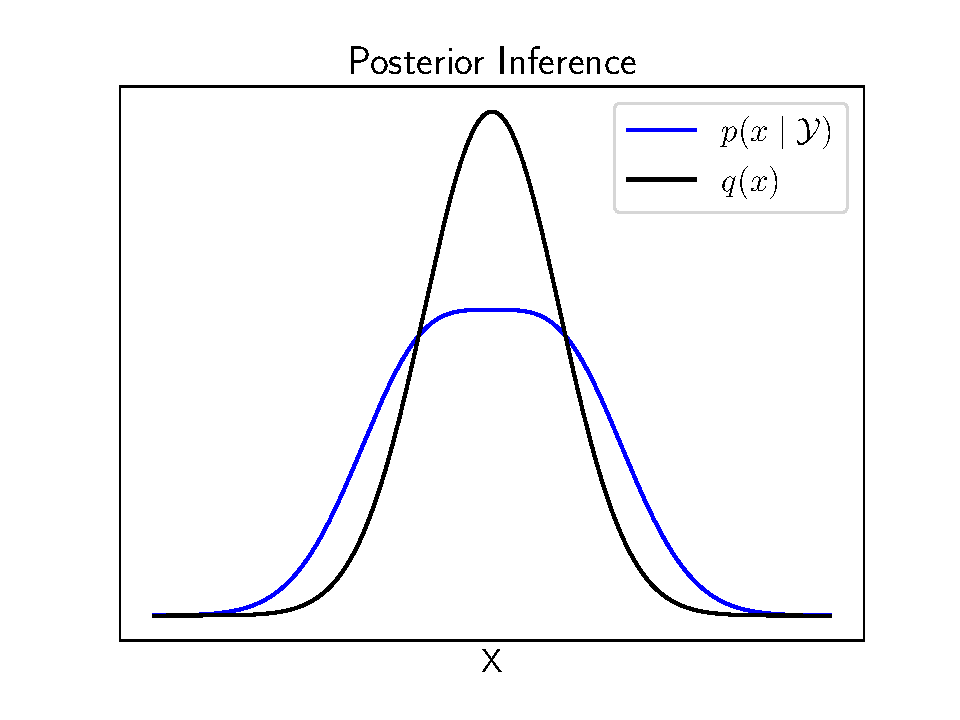
\includegraphics[width=0.29\textwidth]{inf_approx} &
    \hspace{-9mm}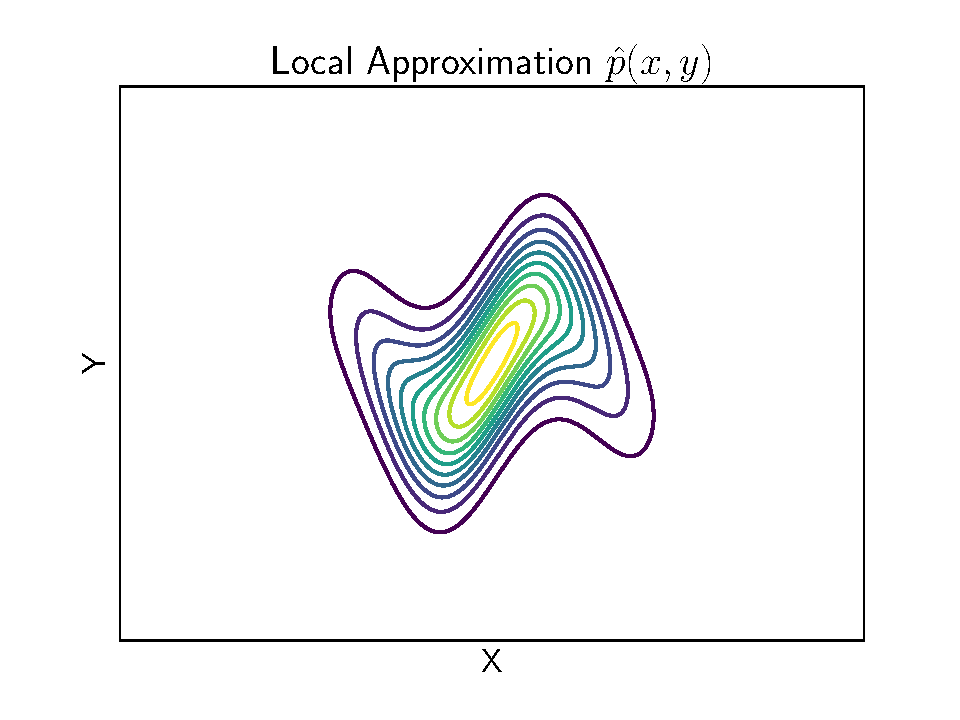
\includegraphics[width=0.29\textwidth]{augmented_dist} &
    \hspace{-9mm}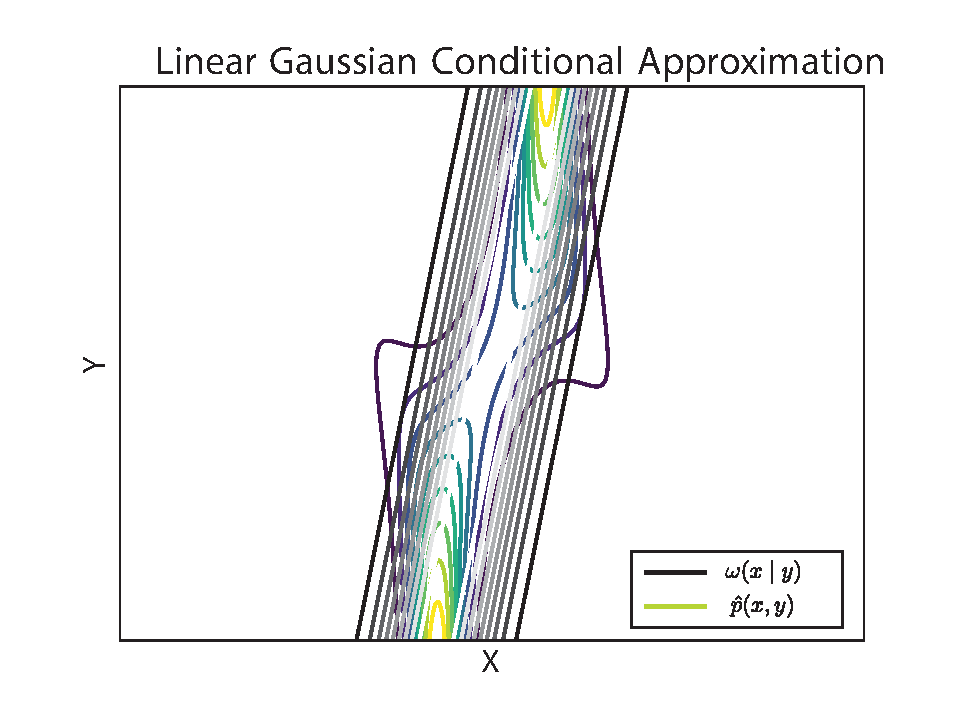
\includegraphics[width=0.29\textwidth]{linear_approx} &
    \hspace{-9mm}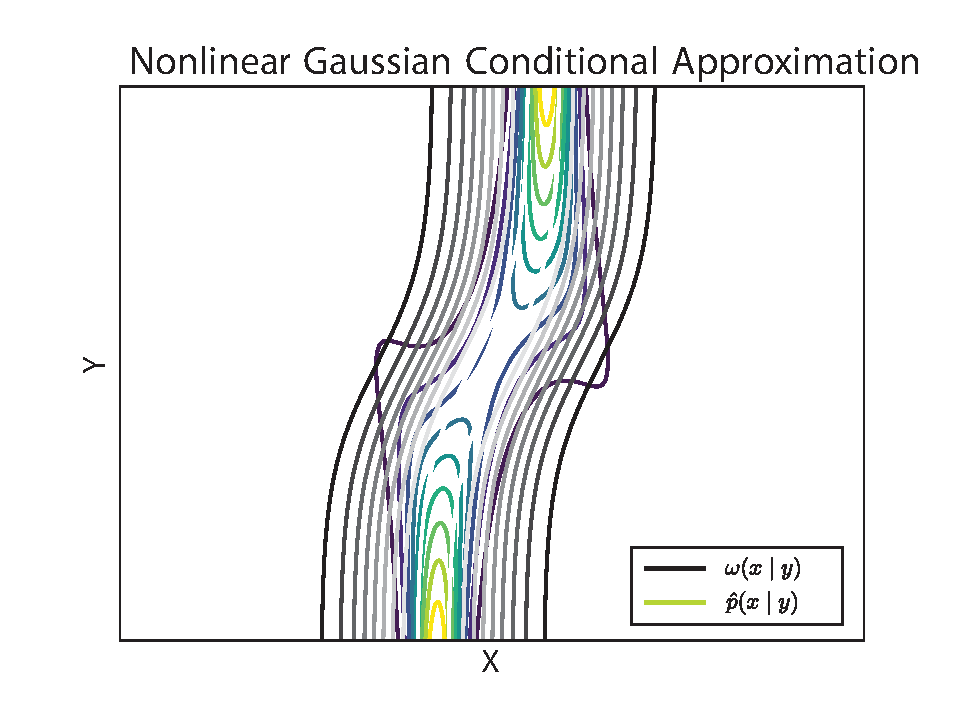
\includegraphics[width=0.29\textwidth]{nonlinear_approx}
  \end{tabular}

  \caption{\small \textbf{Distributional approximations.} \emph{Left:}
  Given observations $\Ycal$ the posterior is approximated with a
  tractable family $q(x) \approx p(x\mid \Ycal)$.  \emph{Center-Left:}
  To consider a new observation $y$, a local approximation is formed
  $\hat{p}(x,y) = q(x) p(y \mid x)$ using the forward model $p(y\mid
  x)$.  \emph{Center-Right:} VIP optimizes a lower bound on MI
  w.r.t.~a distribution $\omega(x\mid y)$ approximating the
  conditional $\hat{p}(x\mid y)$. We use a linear Gaussian
  approximation in this case.  \emph{Right:} Directly parameterizing
  the conditional $\omega(x\mid y)$ allows nonlinear functions of the
  conditioning variable $y$, allowing for better approximations and
  tighter bounds.}

  \label{fig:approx}
\end{figure*}

Given the challenges associated with sample-based estimates of MI, we
shift attention to a more efficient variational approach.  We begin by
introducing the MI bound at the core of VIP and show how this bound
can be extended to sequential decision making.  We then demonstrate
the calculations necessary to apply VIP in a model where observations
are conditionally independent.  We conclude by showing how VIP is
applied in a model of annotations for static data, a common scenario
in the related active learning problem.

\subsection{Variational Information Bound}
Setting aside the details of sequential planning for the moment, we
have that for any valid distribution ${\omega(x\mid y)}$, the following
is a lower bound on MI,
\begin{equation}\label{eq:varmi}
  I(X;Y) \geq H(X) + \EE_p[ \log \omega(X\mid Y) ].
\end{equation}
This well-known bound is the result of Gibbs' inequality, and has been
independently explored in various contexts~\citep{agakov2004algorithm,
  mohamed2015variational, gao2016variational, chen2018learning}.  The
dual problem, then, is to maximize this bound w.r.t.~${\omega(x\mid
  y)}$, which we refer to as the \emph{auxiliary distribution}.


%% This well-known bound is the result of Gibbs' inequality, and has been
%% independently explored for channel coding~\citep{agakov2004algorithm},
%% reinforcement learning~\citep{mohamed2015variational}, and feature
%% selection~\citep{gao2016variational, chen2018learning}.

In the sequential setting, at each planning stage $t$ we require the
posterior mutual information, ${I(X,Y_t\mid \Dcal_{t-1})}$.  Direct application of the
bound~\eqref{eq:varmi} results in,
\[
  H(X\mid \Dcal_{t-1}) + \EE_p[ \log \omega(X\mid Y) \mid \Dcal_{t-1}],
\]
which involves expectations over the posterior distribution ${p(x,y_t
  \mid \Dcal_{t-1})}$.  Thus, application of this bound to sequential
decision making requires further approximation, which we now discuss.

At a high-level, VIP extends the bound~\eqref{eq:varmi} to the
sequential setting through a series of approximating distributions.
First, given past observations and actions $\Dcal_{t-1} =
\{\Acal_{t-1}, \Ycal_{t-1}\}$, we form a variational approximation to
the posterior \mbox{$q(x)\approx p(x\mid \Dcal_{t-1})$}.  Then, we
construct a local approximation over the joint distribution
\mbox{$\hat{p}_a(x,y_t) \approx p(x,y_t\mid \Dcal_{t-1})$} for each
hypothesized action $a=1,\ldots,A$.  Finally, we perform planning by
optimizing a lower bound with respect to an auxiliary
  distribution $\omega(x\mid y_t)$ and select the maximizing action
$a_t$ for the next time step.  See \FIG\ref{fig:approx} for an
illustration.

\subsection{Conditionally Independent Observations}

We begin with the simple model in
\EQN\ref{eq:conditional_indep_joint}, where observations $y$ are
independent conditioned on latent $x$.  Let $\Dcal_{t-1} =
\{\Acal_{t-1}, \Ycal_{t-1}\}$ be the set of past actions and
observations, assume that we have a variational approximation of the
posterior \mbox{$q(x) \approx p(x \mid \Dcal_{t-1})$}.  We then form a
local approximation of the distribution over a future measurement at
time $t$,
\begin{equation}\label{eq:local_approx}
  \hat{p}_{a}(x,y_t) \equiv q_{t-1}(x) p_{a}(y_t \mid x).
\end{equation}
Here, $p_{a}(y_t \mid x)$ is the true likelihood under the
hypothesized action $a$.  The distribution $\hat{p}(\cdot)$ is
analogous to the \emph{augmented distribution} at each stage of EP
inference, which we will exploit in the next section.  We can then
bound the MI under $\hat{p}(\cdot)$ as,
\begin{equation}\label{eq:varmi_approx}
  H_{\hat{p}}(X) + \max_{a, \,\omega}  \;\EE_{\hat{p}_a}\left[ \log \omega(X \mid Y_{t+1})
  \right].
\end{equation}
We have moved the marginal entropy outside the optimization since it is
constant in this model, and so can be ignored for planning.  The bound
can be evaluated in parallel for a discrete set of actions
$1,\ldots,A$.

\FIG\ref{fig:approx} illustrates the role of each approximation in a
single planning stage, and how the approximations relate to the target
distributions.  To be clear, \EQN\eqref{eq:varmi_approx} bounds mutual
information w.r.t.~the local approximate distribution
$\hat{p}(\cdot)$, not MI under the true posterior.  The conditions
under which $\hat{p}(\cdot)$ is a reliable surrogate for posterior MI
are the same as those conditions that must hold for variational
inference to be effective.

\subsection{Annotation Models}\label{sec:annotation}

The conditionally independent model of the previous section is simple
and does not apply in all settings.  Consider a different, more
complicated distribution, often arising in active
learning~\citep{settles2012active}.  Specifically, consider a joint
distribution over latent $x$, data $\{z_d\}_{d=1}^D$ which are fixed,
and annotations $\{y_d\}_{d=1}^D$,
\[
  p(x,y,z) = p(x) \prod_{d=1}^D p(z_d \mid x) p(y_d \mid z_d). 
\]
For example, $y_d$ may be a discrete class assignment for an image
$z_d$.  

The objective at each learning stage selects the most informative
annotation, \mbox{$\max_d I(X;Y_d \mid \Dcal_{t-1})$}, where
$\Dcal_{t-1}$ represents the set of data and previous annotations
after $t-1$ learning rounds.  MI is computed with respect to the
distribution,
\[
  p(x,y_d \mid \Dcal_{t-1}) \propto p(x \mid \Dcal_{t-1} \setminus \{z_d\}) p(z_d \mid
    x ) p(y_d \mid z_d).
\]
Here, $p(x \mid \Dcal_{t-1} \setminus \{z_d\})$ represents the
posterior distribution after removing $z_d$ from the data.  This step
is algebraic, but intuitively avoids double counting $z_d$.

To form a local approximation we appeal to our connection with the EP
augmented distribution.  We assume an EP-like posterior approximation
which is a product of factor approximations (messages): $q(x) \propto
\prod_{d=1}^D \psi_d(x)$.  The \emph{cavity distribution}
$q^{\backslash d}(x) \propto q(x) / \psi_d(x)$ expresses the posterior
approximation having removed $z_d$.  Our local  approximation is then,
\begin{equation}
  \hat{p}(x, y_d) \propto q^{\backslash d}(x) p(z_d \mid x) p(y_d \mid z_d).
\end{equation}
The MI lower bound is then identical to~\eqref{eq:varmi_approx}.  More
complicated models with nuisance variables that must be integrated out
for planning can be handled in the same manner.  We consider such a
setting for labeled LDA active learning example in
Sec.~\ref{sec:llda}.  
